\documentclass[12pt,titlepage]{article}
\usepackage[margin=1.25in]{geometry}
\usepackage{graphicx,amsmath,blindtext,enumitem,minted}

%% Variables definition
\newcommand{\vSubject}{Basic Programming}
\newcommand{\vSubtitle}{Array 2}
\newcommand{\vName}{Dicha Zelianivan Arkana}
\newcommand{\vNIM}{2241720002}
\newcommand{\vClass}{1i}
\newcommand{\vDepartment}{Information Technology}
\newcommand{\vStudyProgram}{D4 Informatics Engineering}

%% [START] Tikz related stuff
\usepackage{tikz}
\usetikzlibrary{svg.path,calc,shapes.geometric,shapes.misc}
\tikzstyle{terminator} = [rectangle, draw, text centered, rounded corners = 1em, minimum height=2em]
\tikzstyle{preparation} = [chamfered rectangle, chamfered rectangle sep=0.75em, draw, text centered, minimum height = 2em]
\tikzstyle{process} = [rectangle, draw, text centered, minimum height=2em]
\tikzstyle{decision} = [diamond, aspect=2, draw, text centered, minimum height=2em]
\tikzstyle{data}=[trapezium, draw, text centered, trapezium left angle=60, trapezium right angle=120, minimum height=2em]
\tikzstyle{connector} = [line width=0.25mm,->]
%% [END] Tikz related stuff

%% [START] Fancy header related stuff
\usepackage{fancyhdr}
\pagestyle{fancy}
\setlength{\headheight}{15pt} % compensate fancyhdr style
\fancyhead{}
\fancyfoot{}
\fancyfoot[L]{\thepage}
\fancyfoot[R]{\textit{\vSubject - \vSubtitle}}
\renewcommand{\footrulewidth}{0.4pt}% default is 0pt, overline for footer
%% [END] Fancy header related stuff

%% [START] Custom tabular command related stuff
\usepackage{tabularx}
\newcommand{\details}[2]{
    #1 & #2  \\
}
%% [END] Custom tabular command related stuff

%% [START] Figure related stuff
\newcommand{\image}[3][1]{
    \begin{figure}[h]
        \centering
        \includegraphics[#1]{#2}
        \caption{#3}
        \label{#3}
    \end{figure}
}
%% [END] Figure related stuff

\begin{document}
\begin{titlepage}
    \centering
    \vfill
    {\bfseries\LARGE
        \vSubject\\
        \vskip0.25cm
        \vSubtitle
    }
    \vfill
    \includegraphics[width=6cm]{images/polinema-logo.png}
    \vfill
    {
        \textbf{Name}\\
        \vName\\
        \vskip0.5cm
        \textbf{NIM}\\
        \vNIM\\
        \vskip0.5cm
        \textbf{Class}\\
        \vClass\\
        \vskip0.5cm
        \textbf{Department}\\
        \vDepartment\\
        \vskip0.5cm
        \textbf{Study Program}\\
        \vStudyProgram
    }
\end{titlepage}

\section*{Assignment}
Adi is a student who every day helps sell cakes made by his mother in the canteen
in several campus buildings where Adi studies. Description: Rows showing the
canteen in a building; Column shows the number of cakes)

\begin{table*}[h]
    \begin{tabular}{|c|c|c|c|c|}
        \hline
        ~ & \textbf{Pancakes} & \textbf{Pudding} & \textbf{Rainbow Cake} & \textbf{Steamed Buns} \\
        \hline
        \textbf{Building A} & 10 & 25 & 20 & 25 \\
        \hline
        \textbf{Building B} & 15 & 23 & 15 & 25 \\
        \hline
        \textbf{Building C} & 12 & 12 & 19 & 23 \\
        \hline
        \textbf{Building D} & 13 & 10 & 28 & 20 \\
        \hline
    \end{tabular}
\end{table*}
The price of a pack of pancakes is IDR 3000, pudding is IDR 2500; rainbow cake is
IDR 4000, and steamed buns is IDR 4500. Create a flowchart to calculate:
\begin{enumerate}[label=\alph*.]
    \item {
        The number of cakes sold in each canteen in buildings A to D

        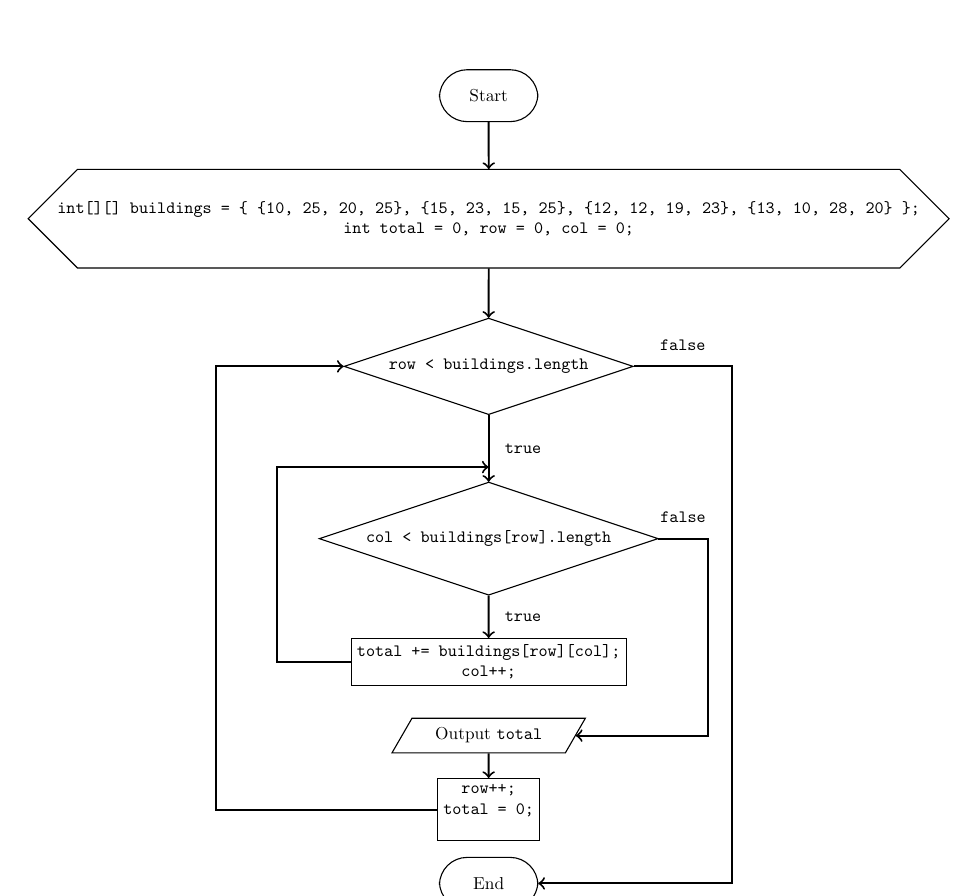
\begin{tikzpicture}[every text node part/.style={align=center}, scale=0.625, every node/.style={scale=0.625}]
            \centering
            \node (start) [terminator, align=center, minimum width=2cm, minimum height=3em] {Start};
            \node (prep) [preparation, below of=start, yshift=-1.5cm, chamfered rectangle sep=1.5em, align=left] {
                \texttt{int[][] buildings = \string{
                    \string{10, 25, 20, 25\string},
                    \string{15, 23, 15, 25\string},
                    \string{12, 12, 19, 23\string},
                    \string{13, 10, 28, 20\string}
                \string};}\\
                \texttt{int total = 0, row = 0, col = 0;}
            };
            \node (cond-1) [decision, below of=prep, yshift=-2cm, aspect=3] {\texttt{row < buildings.length}};
            \node (cond-2) [decision, below of=cond-1, yshift=-2.5cm, aspect=3] {\texttt{col < buildings[row].length}};
            \node (process) [process, below of=cond-2, yshift=-1.5cm, align=center] {
                \texttt{total += buildings[row][col];}\\
                \texttt{col++;}
            };
            \node (output) [data, below of=process, yshift=-5mm] {Output \texttt{total}};
            \node (inc) [process, below of=output, yshift=-5mm, align=center] {
                \texttt{row++;}\\
                \texttt{total = 0;}\\
            };
            \node (end) [terminator, below of=inc, align=center, minimum width=2cm, minimum height=3em, yshift=-5mm] {End};
            \draw [connector] (start) -- (prep);
            \draw [connector] (prep) -- (cond-1);
            \draw [connector] (cond-1.east) -- node[above=2mm] {\texttt{false}} ($(cond-1.east)+(2cm,0)$) |- (end.east);
            \draw [connector] (cond-2.east) -- node[above=2mm] {\texttt{false}} ($(cond-2.east)+(1cm,0)$) |- (output.east);
            \draw [connector] (cond-1) -- node[right=2mm] {\texttt{true}} (cond-2);
            \draw [connector] (cond-2) -- node[right=2mm] {\texttt{true}} (process);
            \draw [connector] (process.west) -- ($(process.west)-(1.5cm,0)$) |- ($(cond-2.north)+(0,3mm)$);
            \draw [connector] (output) -- (inc);
            \draw [connector] (inc.west) -- ($(inc.west)-(4.5cm,0)$) |- (cond-1.west);
        \end{tikzpicture}

        Output: \texttt{80, 78, 66, 71}
    }
    \pagebreak
    \item {
        The number of each cake in the whole building
    
        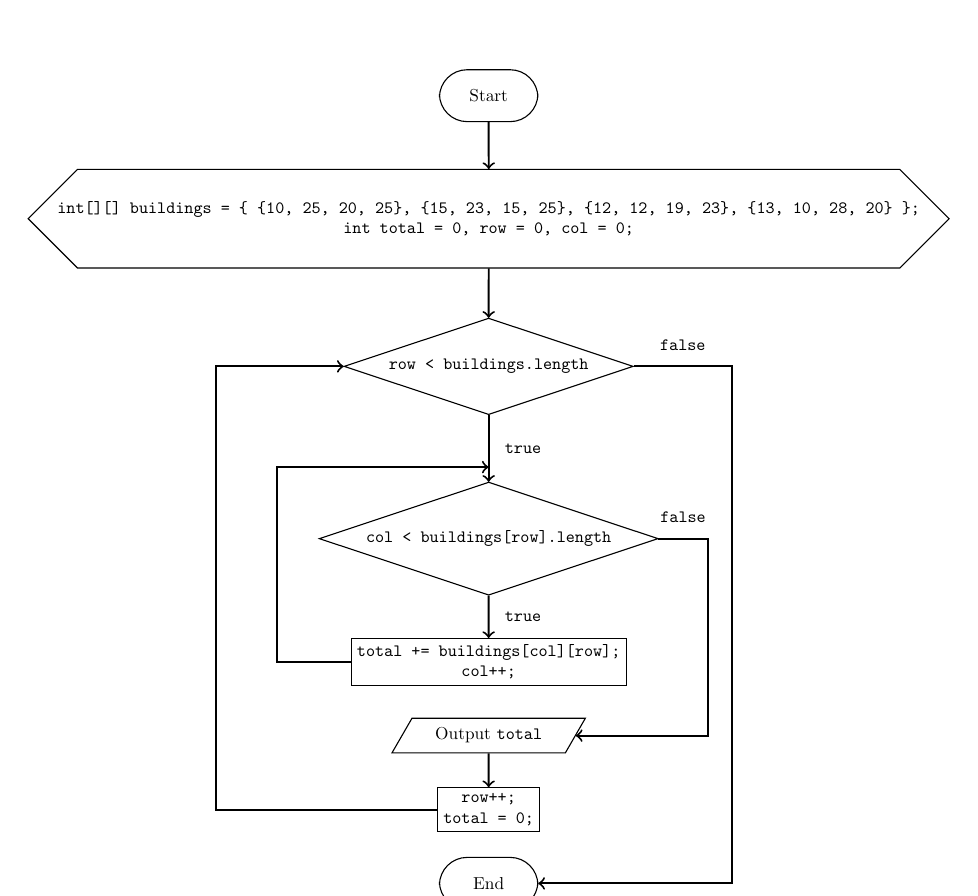
\begin{tikzpicture}[every text node part/.style={align=center}, scale=0.625, every node/.style={scale=0.625}]
            \centering
            \node (start) [terminator, align=center, minimum width=2cm, minimum height=3em] {Start};
            \node (prep) [preparation, below of=start, yshift=-1.5cm, chamfered rectangle sep=1.5em, align=left] {
                \texttt{int[][] buildings = \string{
                    \string{10, 25, 20, 25\string},
                    \string{15, 23, 15, 25\string},
                    \string{12, 12, 19, 23\string},
                    \string{13, 10, 28, 20\string}
                \string};}\\
                \texttt{int total = 0, row = 0, col = 0;}
            };
            \node (cond-1) [decision, below of=prep, yshift=-2cm, aspect=3] {\texttt{row < buildings.length}};
            \node (cond-2) [decision, below of=cond-1, yshift=-2.5cm, aspect=3] {\texttt{col < buildings[row].length}};
            \node (process) [process, below of=cond-2, yshift=-1.5cm, align=center] {
                \texttt{total += buildings[col][row];}\\
                \texttt{col++;}
            };
            \node (output) [data, below of=process, yshift=-5mm] {Output \texttt{total}};
            \node (inc) [process, below of=output, yshift=-5mm, align=center] {
                \texttt{row++;}\\
                \texttt{total = 0;}
            };
            \node (end) [terminator, below of=inc, align=center, minimum width=2cm, minimum height=3em, yshift=-5mm] {End};
            \draw [connector] (start) -- (prep);
            \draw [connector] (prep) -- (cond-1);
            \draw [connector] (cond-1.east) -- node[above=2mm] {\texttt{false}} ($(cond-1.east)+(2cm,0)$) |- (end.east);
            \draw [connector] (cond-2.east) -- node[above=2mm] {\texttt{false}} ($(cond-2.east)+(1cm,0)$) |- (output.east);
            \draw [connector] (cond-1) -- node[right=2mm] {\texttt{true}} (cond-2);
            \draw [connector] (cond-2) -- node[right=2mm] {\texttt{true}} (process);
            \draw [connector] (process.west) -- ($(process.west)-(1.5cm,0)$) |- ($(cond-2.north)+(0,3mm)$);
            \draw [connector] (output) -- (inc);
            \draw [connector] (inc.west) -- ($(inc.west)-(4.5cm,0)$) |- (cond-1.west);
        \end{tikzpicture}

        Output: \texttt{50, 70, 82, 93}
    }
    \pagebreak
    \item {
        Total profit if all the cakes in each buildings are sold out

        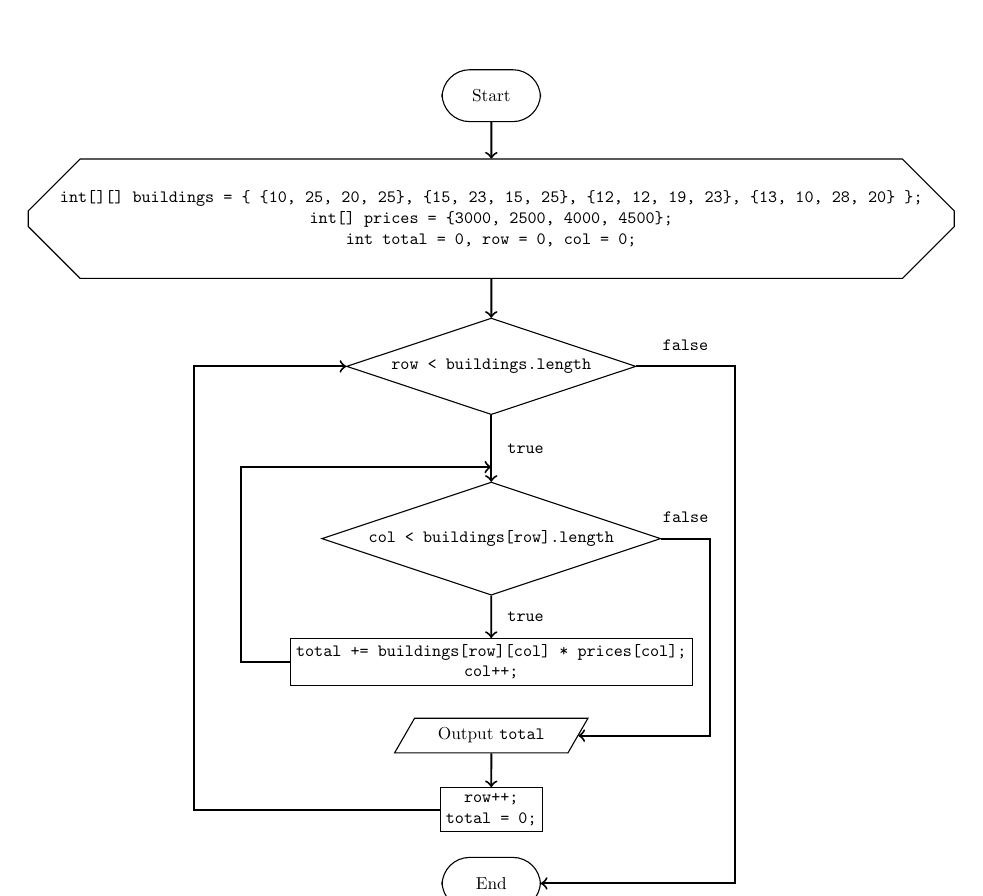
\begin{tikzpicture}[every text node part/.style={align=center}, scale=0.625, every node/.style={scale=0.625}]
            \centering
            \node (start) [terminator, align=center, minimum width=2cm, minimum height=3em] {Start};
            \node (prep) [preparation, below of=start, yshift=-1.5cm, chamfered rectangle sep=1.5em, align=left] {
                \texttt{int[][] buildings = \string{
                    \string{10, 25, 20, 25\string},
                    \string{15, 23, 15, 25\string},
                    \string{12, 12, 19, 23\string},
                    \string{13, 10, 28, 20\string}
                \string};}\\
                \texttt{int[] prices = \string{3000, 2500, 4000, 4500\string};}\\
                \texttt{int total = 0, row = 0, col = 0;}
            };
            \node (cond-1) [decision, below of=prep, yshift=-2cm, aspect=3] {\texttt{row < buildings.length}};
            \node (cond-2) [decision, below of=cond-1, yshift=-2.5cm, aspect=3] {\texttt{col < buildings[row].length}};
            \node (process) [process, below of=cond-2, yshift=-1.5cm, align=center] {
                \texttt{total += buildings[row][col] * prices[col];}\\
                \texttt{col++;}
            };
            \node (output) [data, below of=process, yshift=-5mm] {Output \texttt{total}};
            \node (inc) [process, below of=output, yshift=-5mm, align=center] {
                \texttt{row++;}\\
                \texttt{total = 0;}
            };
            \node (end) [terminator, below of=inc, align=center, minimum width=2cm, minimum height=3em, yshift=-5mm] {End};
            \draw [connector] (start) -- (prep);
            \draw [connector] (prep) -- (cond-1);
            \draw [connector] (cond-1.east) -- node[above=2mm] {\texttt{false}} ($(cond-1.east)+(2cm,0)$) |- (end.east);
            \draw [connector] (cond-2.east) -- node[above=2mm] {\texttt{false}} ($(cond-2.east)+(1cm,0)$) |- (output.east);
            \draw [connector] (cond-1) -- node[right=2mm] {\texttt{true}} (cond-2);
            \draw [connector] (cond-2) -- node[right=2mm] {\texttt{true}} (process);
            \draw [connector] (process.west) -- ($(process.west)-(1cm,0)$) |- ($(cond-2.north)+(0,3mm)$);
            \draw [connector] (output) -- (inc);
            \draw [connector] (inc.west) -- ($(inc.west)-(5cm,0)$) |- (cond-1.west);
        \end{tikzpicture}

        Output: \texttt{285000, 275000, 245500, 266000}
    }
\end{enumerate}

\end{document}

